\documentclass{beamer}
\usepackage[utf8]{}
\usepackage{hyperref}
\usepackage[T1]{fontenc}
\usepackage{tikz}
\usepackage{listings}
\usepackage{algorithm,algorithmic}
\usepackage{amsmath}
\usepackage{pifont}
\usepackage{color}
\usepackage{colortbl}
\usepackage[
    type={CC},
    modifier={by-nc},
    version={4.0},
    imageposition = right
]{doclicense}
\usepackage{ragged2e}
\usepackage{Wue}

\colorlet{shadecolor}{gray!40}

\usepackage{wrapfig}

\renewcommand{\algorithmicrequire}{\textbf{Input:}}
\renewcommand{\algorithmicensure}{\textbf{Output:}}

\setbeamertemplate{itemize items}[square] 
\usepackage[backend=biber,style=numeric-comp,sorting=none]{biblatex}


\author{Di Battista Mattia}
\title{Dual-Based Procedure and Subgradient method implementations}
\institute{Università degli Studi di Roma "Tor Vergata"} 

\usefonttheme[onlymath]{serif}

\begin{document}

\defverbatim[colored]\lstI{
\begin{lstlisting}[language=Python,basicstyle=\footnotesize\ttfamily,keywordstyle=\color{blue}, xleftmargin=.25\textwidth,xrightmargin=.75\textwidth]
self.model.Params.Method = 0
\end{lstlisting}
}

\defverbatim[colored]\lstII{
\begin{lstlisting}[language=Python,keywordstyle=\color{blue},basicstyle=\footnotesize\ttfamily,xleftmargin=.1\textwidth,xrightmargin=.75\textwidth]
self.model.setParam(gp.GRB.Param.Presolve, 0)
self.model.setParam(gp.GRB.Param.Heuristics, 0)
self.model.setParam(gp.GRB.Param.Cuts, 0)
\end{lstlisting}
}

\defverbatim[colored]\lstIII{
\begin{lstlisting}[language=Python,basicstyle=\footnotesize\ttfamily,keywordstyle=\color{blue},xleftmargin=.35\textwidth,xrightmargin=.75\textwidth]
self.model.relax()
\end{lstlisting}
}

\defverbatim[colored]\lstVI{
\begin{lstlisting}[language=Python,basicstyle=\footnotesize\ttfamily,keywordstyle=\color{blue},xleftmargin=.1\textwidth,xrightmargin=.75\textwidth]
self.model.setObjective(obj_func, gp.GRB.MINIMIZE)
self.model.optimize()
return self.model.objVal
\end{lstlisting}
}

    
	\begin{frame}
    \titlepage
    \centering
    \doclicenseIcon
    \end{frame}

	
	\begin{frame}{Outline}
		\tableofcontents
	\end{frame}
	
	\section{Goal}
		    \begin{frame}{Goal}
		    
		    The aim is to implement and evaluate: 
		    
		    \begin{itemize}
		        \item \textbf{Dual-Based Procedure} for \textit{Uncapacitated Facility Location} (UFL)
		        \item \textbf{Subgradient method} for \textit{Lagrangian relaxation}\pause
		    \end{itemize} 
		    Using:
		      \begin{itemize}
		        \item w.r.t. \textit{Linear relaxation} and \textit{Primal Simplex}
		        \item \textit{Python} as programming language
		        \item \textit{Gurobi API}
		    \end{itemize}
		    
		    \end{frame}
		    
	\section{Methodology}
	    
	    \subsection{Primal Simplex}
	    \begin{frame}{Primal Simplex}
        
        \textbf{Main commands} used:
        \begin{itemize}
            \item to set the \textit{Primal Simplex} as solution algorithm:
            \begin{center}
            \lstI
            \end{center}
            
        \item to disable presolve, cut generation and heuristics options:
        
        \lstII
        
        \item to use \textit{Linear relaxation}:
        
        \lstIII
        
        \end{itemize}
	    \end{frame}
	    
	    \subsection{Dual-Based Procedure}
	    \begin{frame}{Dual-Based Procedure (1)}
	    
	       \textit{Uncapacitated Facility Location} \textbf{formulation}:
	     
	     \begin{center}
	     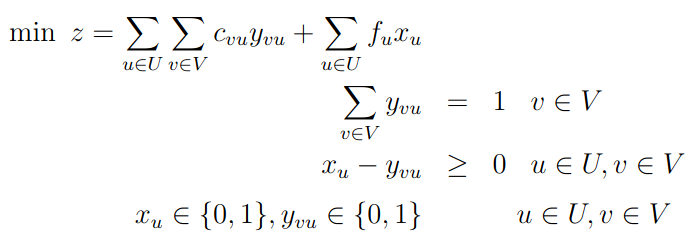
\includegraphics[width=.8\textwidth]{img/algo_1.png}
	     \end{center}
	     
	     \textit{Uncapacitated Facility Location} \textbf{dual formulation}:
	     
	     \begin{center}
	     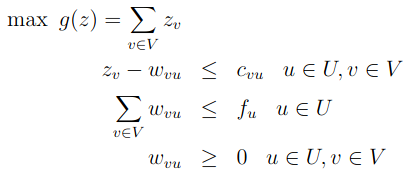
\includegraphics[width=.60\textwidth]{img/algo_2.png}
	     \end{center}
	    
	    \end{frame}
	    
	    \begin{frame}{Dual-Based Procedure (2)}
	   
	   \begin{columns}
	      
	      \column{.4\textwidth}
	      
	      \textbf{Dualoc-Based procedure} (created by \textit{D. Erlenkotter} in \textit{1978})
	      \begin{itemize}
	          \item starting from the dual problem
	          \item provides a \textbf{lower bound} for the primal problem
	          \item high quality and efficiently
	          \item cons: influenced by the sorting of variables
	      \end{itemize}
	      
	      \column{.6\textwidth}
	            \begin{algorithm}[H]
                \begin{algorithmic}[1]
    
                \FOR{$v \in V$}
                \STATE $\bar{z}_{v} = min_{u \in U}\{c_{uv}\}$
                \ENDFOR
                
                \FOR{$s \in V$}
                
                \STATE $\bar{w}_{uv} = max\{0, \bar{z}_{v} - c_{vu}\}$
	            \STATE $z^{max}_{s} = min_{\substack{u \in U}} \{{c_{su} + f_{u}} - \sum_{\substack{v \neq s}} \bar{w}_{vu}\}$
                \ENDFOR
                \RETURN $z^{max}$
                
                \end{algorithmic}
                \caption{}
                \end{algorithm}
	           
	           \end{columns}
	    \end{frame}
	    
	    \subsection{Subgradient method}
	    
	    \begin{frame}{Subgradient method (1)}
	        
	        \textit{Uncapacitated Facility Location} \textbf{formulation}:
	             \begin{center}
               
                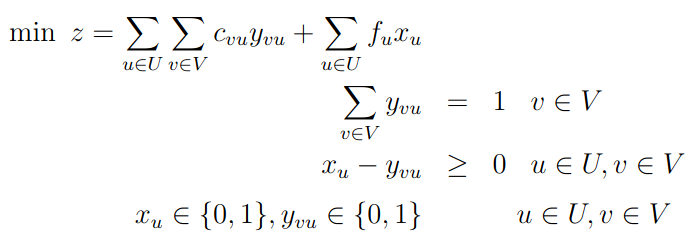
\includegraphics[width=.85\textwidth]{img/algo_1.png}
        	     \end{center}
        	     
        	  \textit{Uncapacitated Facility Location} \textbf{Lagrangian relaxation formulation}:
        	     \begin{center}
        	         
        	         $min \ z = \sum_{\substack{u \in U}} (f_u - \sum_{\substack{v \in V}} \lambda_{uv}) x_u + \sum_{\substack{u \in U}} \sum_{\substack{v \in V}} (c_{uv} + \lambda_{uv}) y_{uv}$
        	         

        	         $\sum_{u \in U} y_{uv} = 1, \ \forall v \in V$
        	         
        	         $x, y \in \{0,1\}$
        	     \end{center}
	    \end{frame}
    
    
    \begin{frame}{Subgradient method (2)}
        
        \begin{columns}
	      
	      \column{.4\textwidth}
	      
	      \textbf{Subgradient method} provides a vector multiplier for \textit{Lagrangian relaxation}
	      \begin{itemize}
	          \item proved its convergence to the optimal \textit{Lagrangian} multiplier
	          \item considering a feasible solution of the \textit{UFL} problem (i.e., \textit{B})
	      \end{itemize}
    
        \column{.6\textwidth}
        
        \begin{algorithm}[H]
                \begin{algorithmic}[1]
    
                \STATE find $x^{(h)}$ in \textit{Lagrangian} problem
                \STATE $s^{(h)} = b - Ax^{(h)}$
                \IF{$s^{(h)} == 0$}{STOP}
                \ENDIF
                \STATE $\theta^{(h)} = \frac{B-L(\lambda^{(h-1)})}{||s^{(h)}||^2}$
                \STATE $\lambda^{(h+1)} = \lambda^{(h)} + \theta^{(h)}\frac{s^{(h)}}{||s^{(h)}||}$
                \STATE $h=h+1$
                \IF{lower bound did not enhance in the last $K$ iterations}{STOP}
                \ENDIF
                
                \end{algorithmic}
                \caption{}
                \end{algorithm}
        \end{columns}
        
        \end{frame}
        
        \begin{frame}{Subgradient method (3)}
            
        \textbf{Assumptions} in the implementation:
        
        \begin{itemize}
        \item started from a \textit{Lagrangian relaxation} solution
        \begin{itemize}
            \item[\ding{113}] randomly generated multiplier 
        \end{itemize}
        \item iterations (i.e., \textit{K}) equal to \textit{100}
        \item \textit{B} equals to the  \textit{Simplex Primal} solution
        \begin{itemize}
            \item[\ding{113}] i.e., the best solution
        \end{itemize}
        \lstVI
        \end{itemize}
        \end{frame}
               
	\section{Performance Evaluation}
	
	\begin{frame}{Performance Evaluation (1)}

	Parameters considered in the \textbf{tests}:
	
	\begin{itemize}
	    \item $(customers;facilities) \in \{(30; 30), (29; 5), (5;29)\}$
	    \item $algorithm \in \{Dualoc, Linear \ relaxation, Lagrangian \  relaxation\}$ 
	    \item ratios:
	    \begin{itemize}
	        \item[\ding{113}] $setup \ cost \approx shipping \ cost$
	        \item[\ding{113}] $setup \ cost \gg shipping \ cost$
	        \item[\ding{113}] $setup \ cost \ll shipping \ cost$
	        \item[\ding{113}] $Var(setup \ cost) \gg Var(shipping \ cost)$
            \item[\ding{113}] $Var(setup \ cost) \ll Var(shipping \ cost)$
	    \end{itemize}
	   \item trials equal to \textit{100} 
	\end{itemize}\pause
	
	\centering
	\textit{4500} \textbf{instances} resolved!
	
	\end{frame}
	
		\begin{frame}{Performance Evaluation (2)}

		Generated \textit{15} \textbf{charts}:
		\begin{enumerate}
		    \item computation time
		    \item percentage error w.r.t \textit{Primal Simplex} solution:
		    \begin{equation}
		    \frac{|Experimental \ Value-Theoretical \ Value|}{Theoretical \ value} \cdot 100
		    \end{equation}
		\end{enumerate}
		
        \end{frame}
	
        \subsection{Dualoc \& Linear relaxation}
	
	    \begin{frame}{Dualoc \& Linear relaxation (1)}
	  
	  \textbf{Test Case 1}: $setup \ cost \approx shipping \ cost$
  
	   \begin{columns}
	   \centering
        \column{.5\textwidth}
        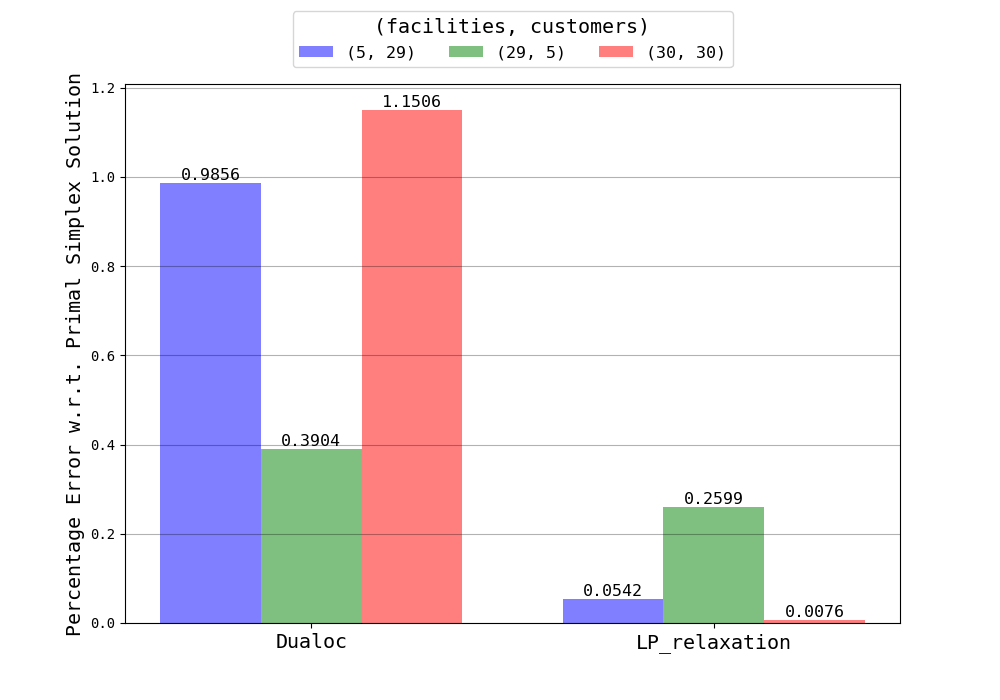
\includegraphics[width=6.5cm,height=4.2cm]{img/chart_error_0.png}
        
        \centering
        \column{.5\textwidth}
        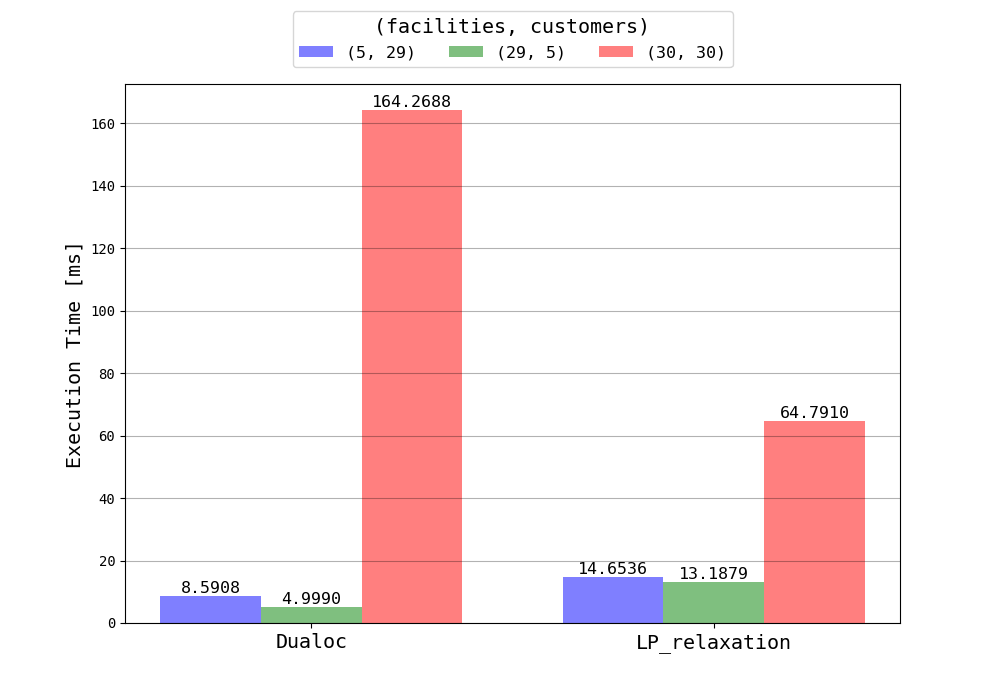
\includegraphics[width=6.5cm,height=4.2cm]{img/chart_time_0.png}
        \end{columns}
	   
	    \end{frame}
	       
	   \begin{frame}{Dualoc \& Linear relaxation (2)}
	    
        \textbf{Test Case 2}: $setup \ cost \gg shipping \ cost$
        
        \begin{columns}
	   \centering
        \column{.5\textwidth}
        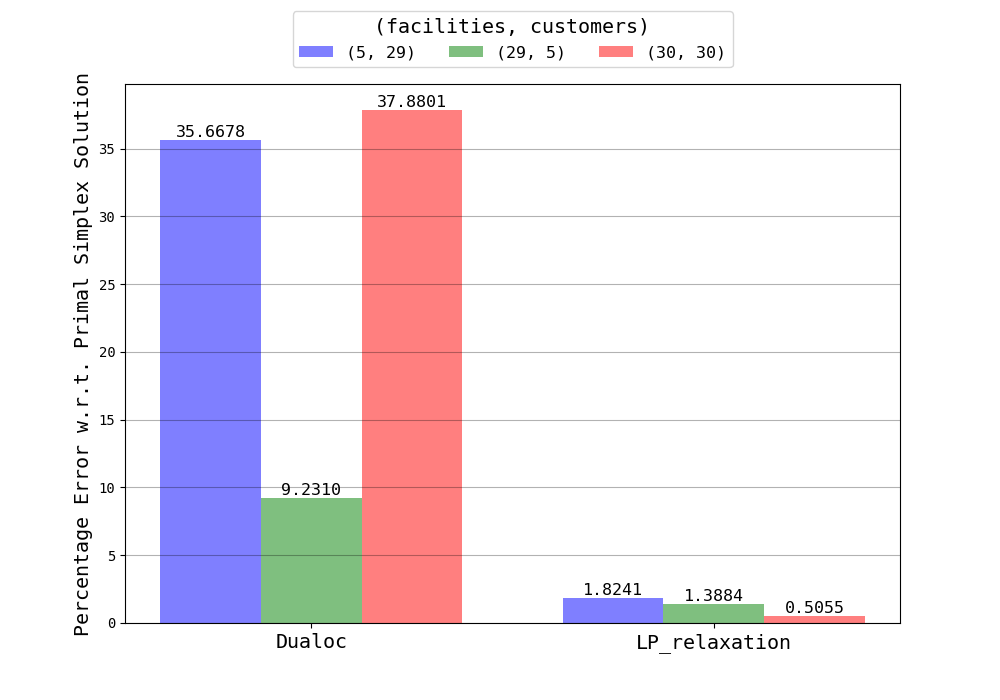
\includegraphics[width=6.5cm,height=4.2cm]{img/chart_error_1.png}
        
        \centering
        \column{.5\textwidth}
        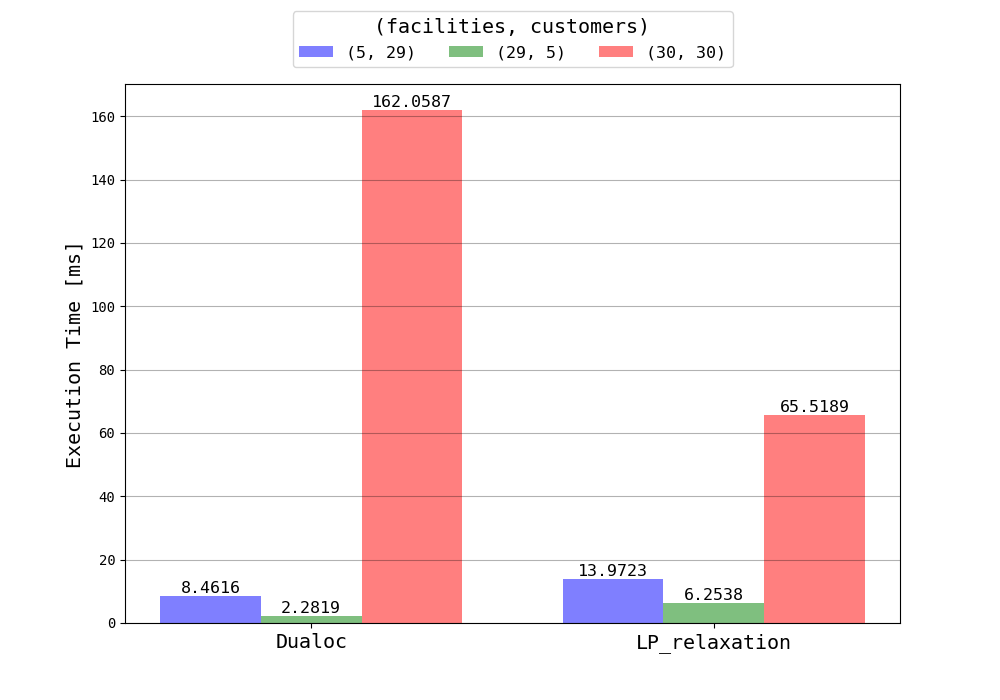
\includegraphics[width=6.5cm,height=4.2cm]{img/chart_time_1.png}
        \end{columns}
        
	    \end{frame}
	    
	    \begin{frame}{Dualoc \& Linear relaxation (3)}
	    
        \textbf{Test Case 3}: $setup \ cost \ll shipping \ cost$
        
        
        \begin{columns}
	   \centering
        \column{.5\textwidth}
        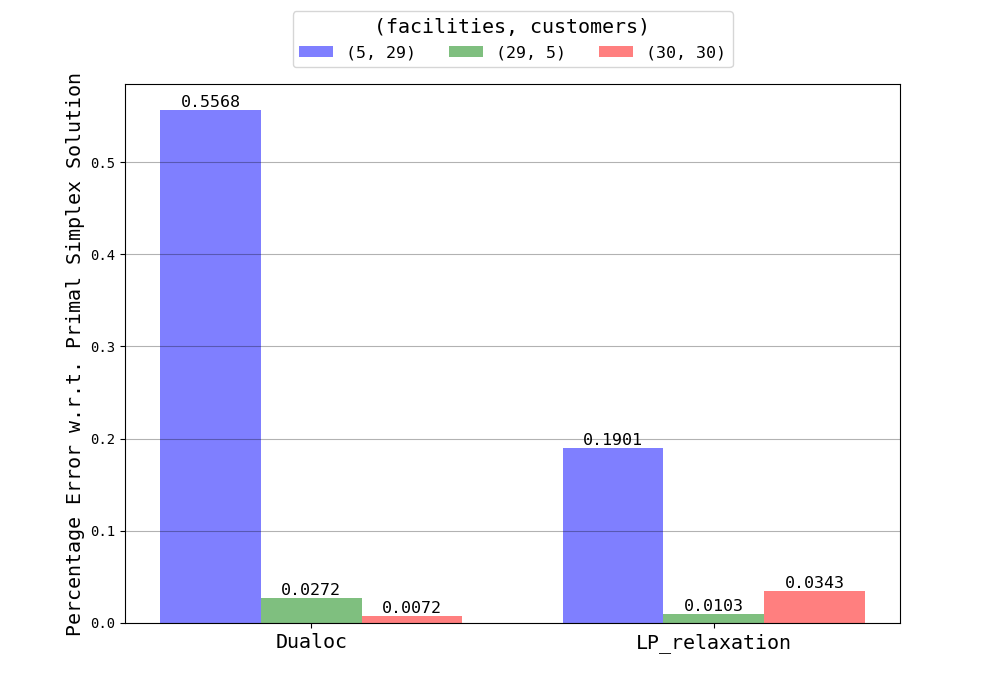
\includegraphics[width=6.5cm,height=4.2cm]{img/chart_error_2.png}
        
        \centering
        \column{.5\textwidth}
        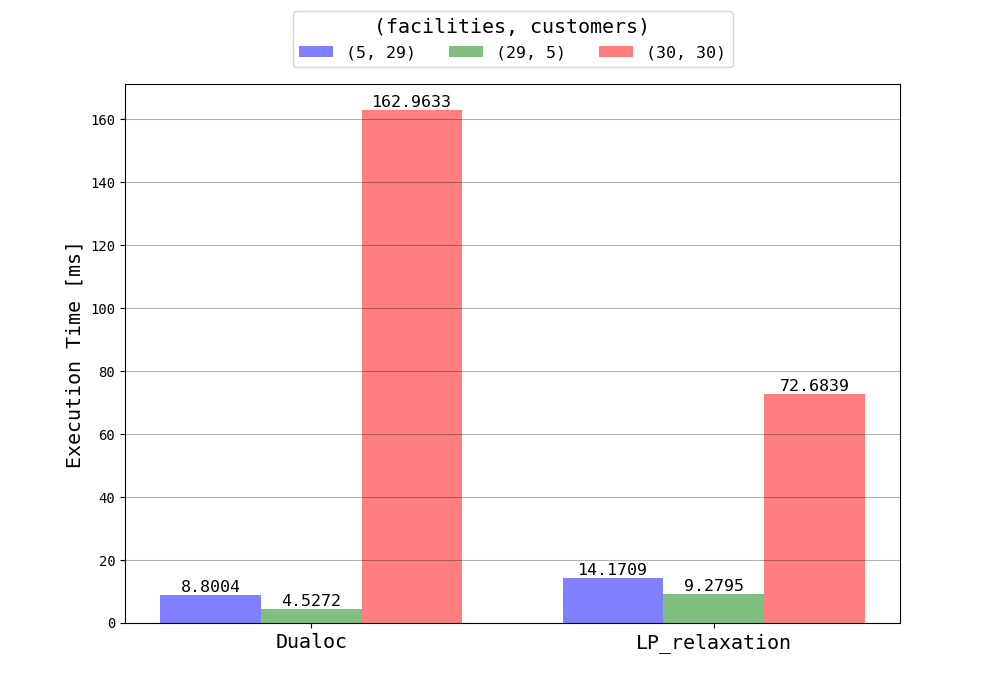
\includegraphics[width=6.5cm,height=4.2cm]{img/chart_time_2.png}
        \end{columns}
        
	    \end{frame}
	    
	    \begin{frame}{Dualoc \& Linear relaxation (4)}
	    
        \textbf{Test Case 4}: $Var(setup \ cost) \gg Var(shipping \ cost)$
        
        
        \begin{columns}
	   \centering
        \column{.5\textwidth}
        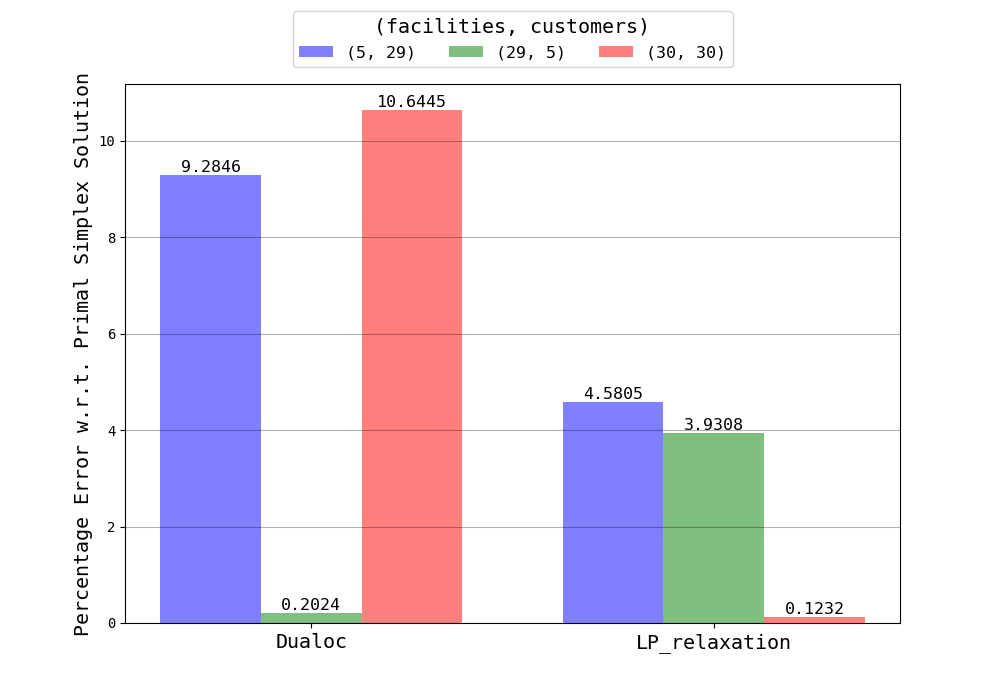
\includegraphics[width=6.5cm,height=4.2cm]{img/chart_error_3.png}
        
        \centering
        \column{.5\textwidth}
        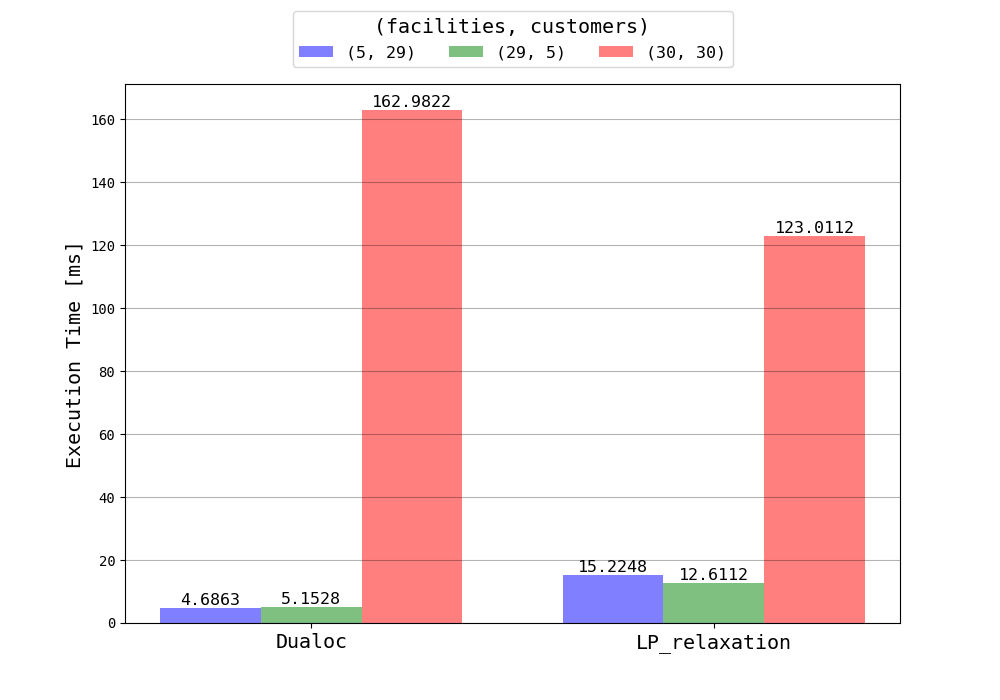
\includegraphics[width=6.5cm,height=4.2cm]{img/chart_time_3.png}
        \end{columns}
        
	    \end{frame}
	    
	    \begin{frame}{Dualoc \& Linear relaxation (5)}
	    
        \textbf{Test Case 5}: $Var(setup \ cost) \ll Var(shipping \ cost)$
        
        
        \begin{columns}
	   \centering
        \column{.5\textwidth}
        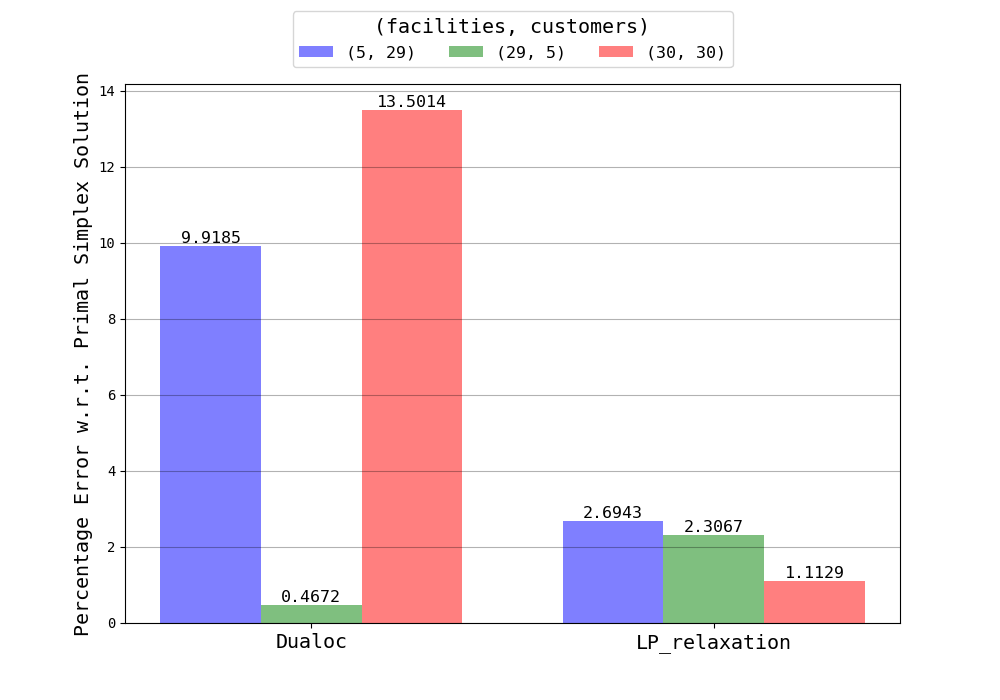
\includegraphics[width=6.5cm,height=4.2cm]{img/chart_error_4.png}
        
        \centering
        \column{.5\textwidth}
        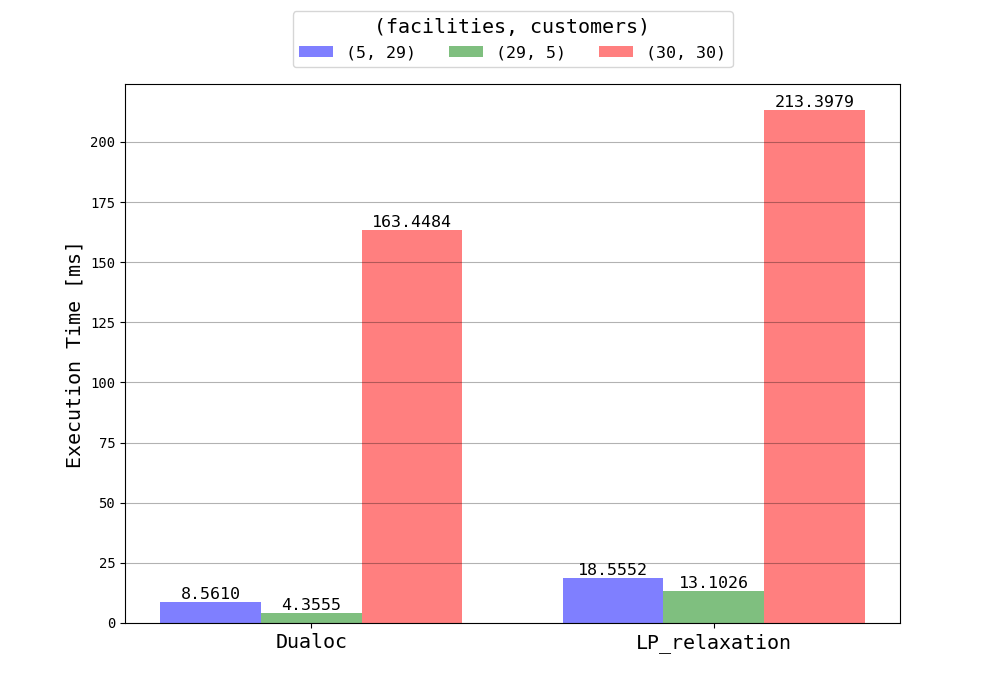
\includegraphics[width=6.5cm,height=4.2cm]{img/chart_time_4.png}
        \end{columns}
        
	    \end{frame}
	    
	    \subsection{Lagrangian relaxation}
	    
	    \begin{frame}{Lagrangian relaxation (1)}
	  
	  \textbf{Test Case 1}: $setup \ cost \approx shipping \ cost$
  
	   \begin{columns}
	   \centering
        \column{.5\textwidth}
        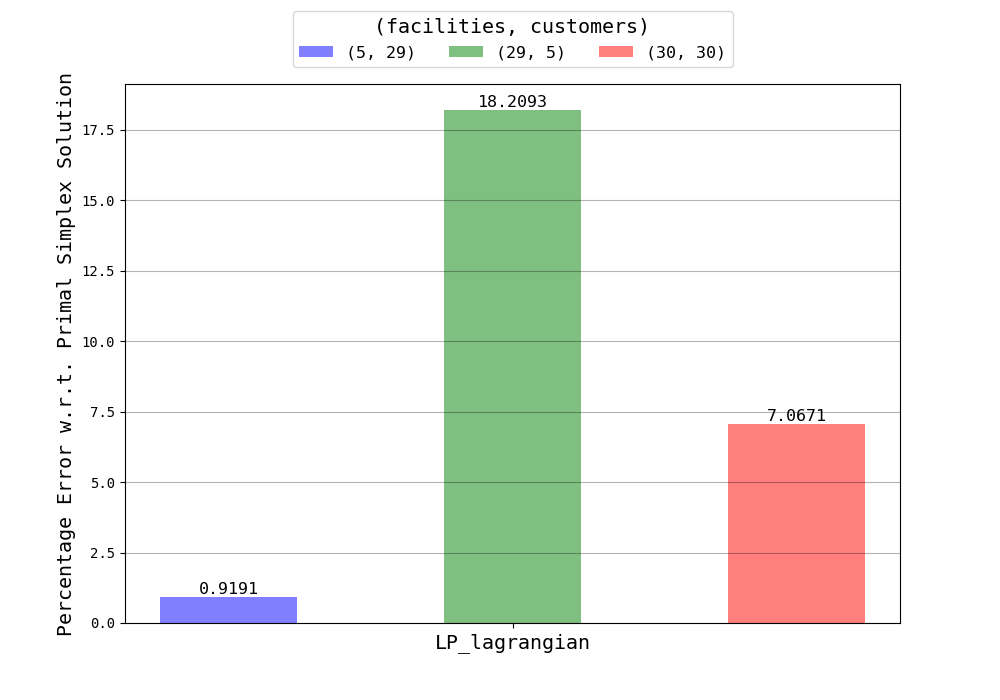
\includegraphics[width=6.5cm,height=4.2cm]{img/chart_error_lagrangian_0.png}
        
        \centering
        \column{.5\textwidth}
        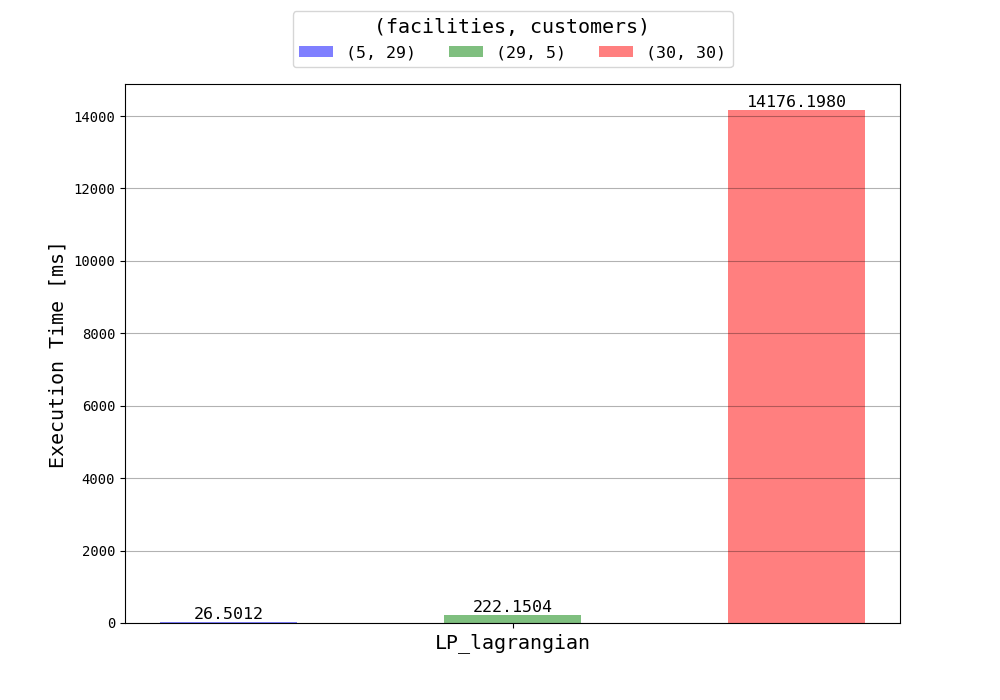
\includegraphics[width=6.5cm,height=4.2cm]{img/chart_time_lagrangian_0.png}
        \end{columns}
	   
	    \end{frame}
	       
	   \begin{frame}{Lagrangian relaxation (2)}
	    
        \textbf{Test Case 2}: $setup \ cost \gg shipping \ cost$
        
        \begin{columns}
	   \centering
        \column{.5\textwidth}
        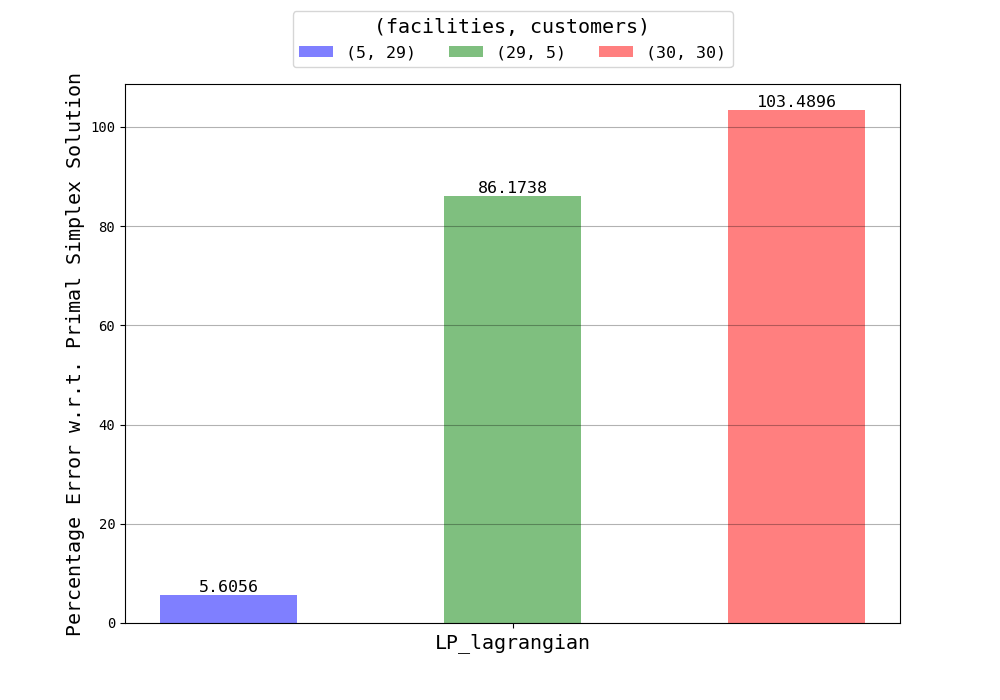
\includegraphics[width=6.5cm,height=4.2cm]{img/chart_error_lagrangian_1.png}
        
        \centering
        \column{.5\textwidth}
        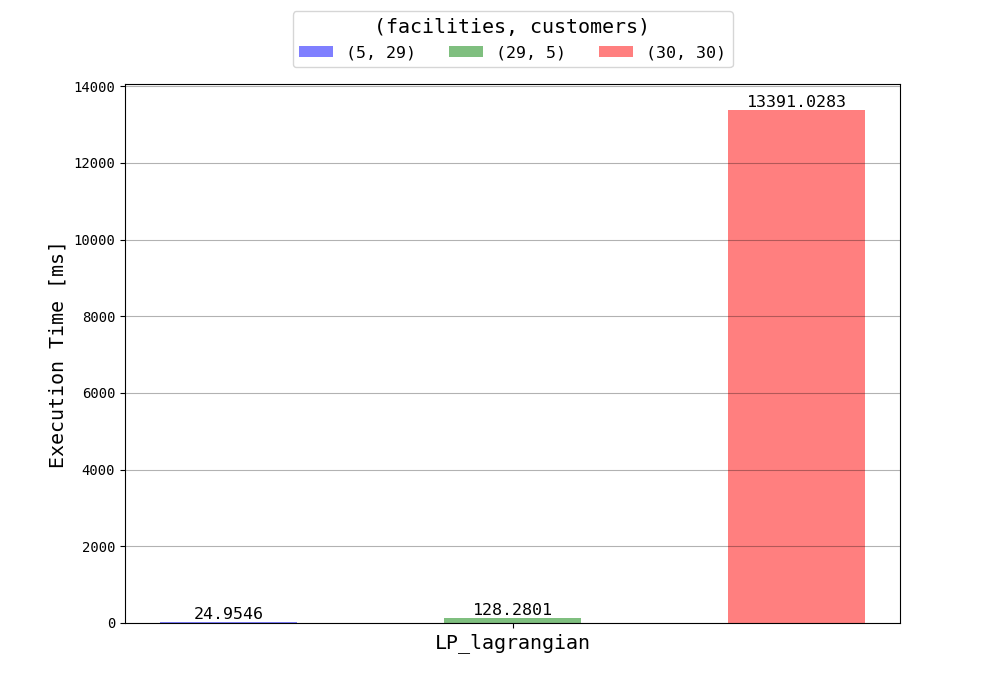
\includegraphics[width=6.5cm,height=4.2cm]{img/chart_time_lagrangian_1.png}
        \end{columns}
        
	    \end{frame}
	    
	    \begin{frame}{Lagrangian relaxation (3)}
	    
        \textbf{Test Case 3}: $setup \ cost \ll shipping \ cost$
        
        
        \begin{columns}
	   \centering
        \column{.5\textwidth}
        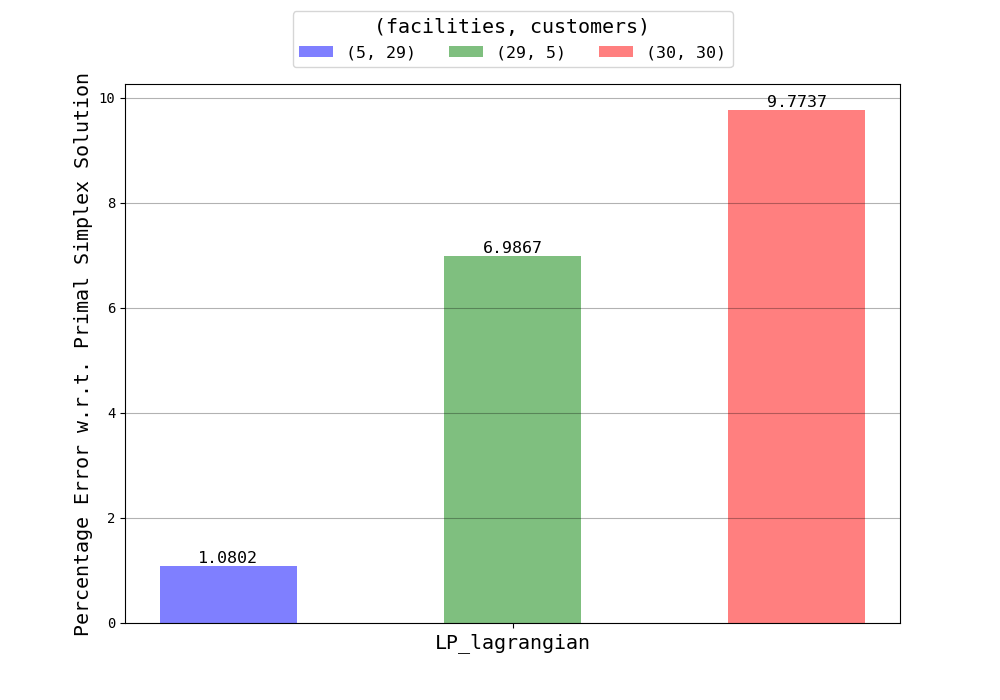
\includegraphics[width=6.5cm,height=4.2cm]{img/chart_error_lagrangian_2.png}
        
        \centering
        \column{.5\textwidth}
        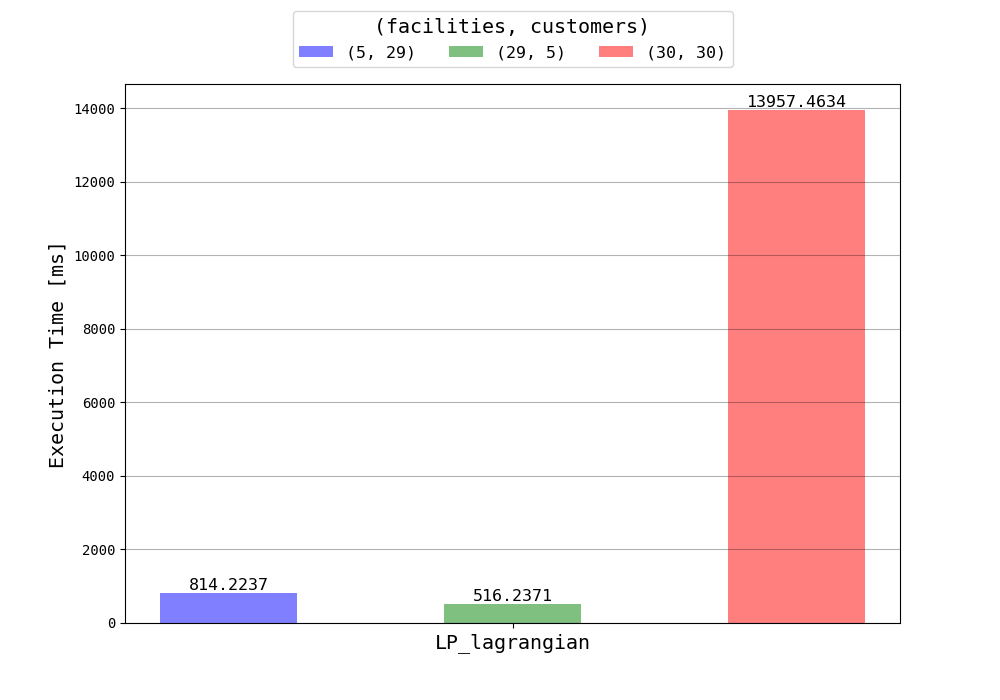
\includegraphics[width=6.5cm,height=4.2cm]{img/chart_time_lagrangian_2.png}
        \end{columns}
        
	    \end{frame}
	    
	    \begin{frame}{Lagrangian relaxation (4)}
	    
        \textbf{Test Case 4}: $Var(setup \ cost) \gg Var(shipping \ cost)$
        
        
        \begin{columns}
	   \centering
        \column{.5\textwidth}
        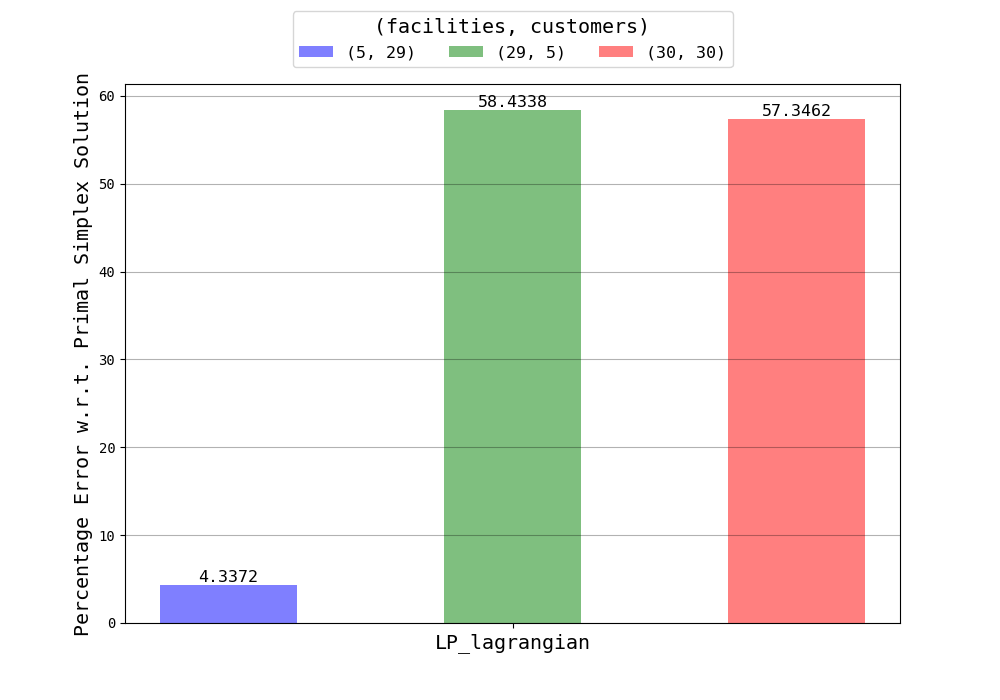
\includegraphics[width=6.5cm,height=4.2cm]{img/chart_error_lagrangian_3.png}
        
        \centering
        \column{.5\textwidth}
        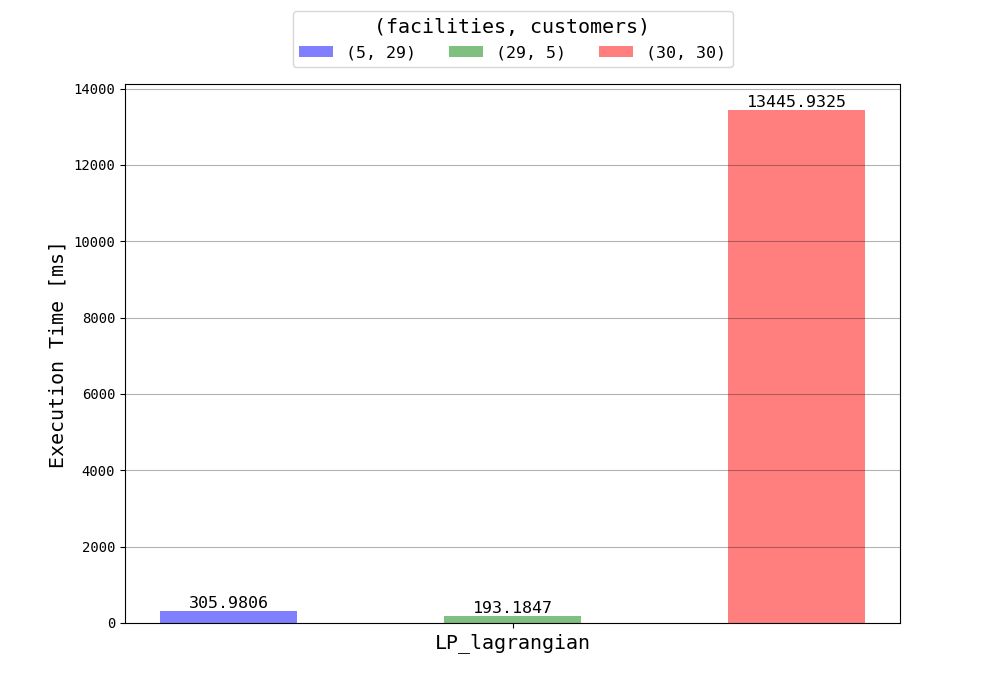
\includegraphics[width=6.5cm,height=4.2cm]{img/chart_time_lagrangian_3.png}
        \end{columns}
        
	    \end{frame}
	    
	    \begin{frame}{Lagrangian relaxation (5)}
	    
        \textbf{Test Case 5}: $Var(setup \ cost) \ll Var(shipping \ cost)$
        
        
        \begin{columns}
	   \centering
        \column{.5\textwidth}
        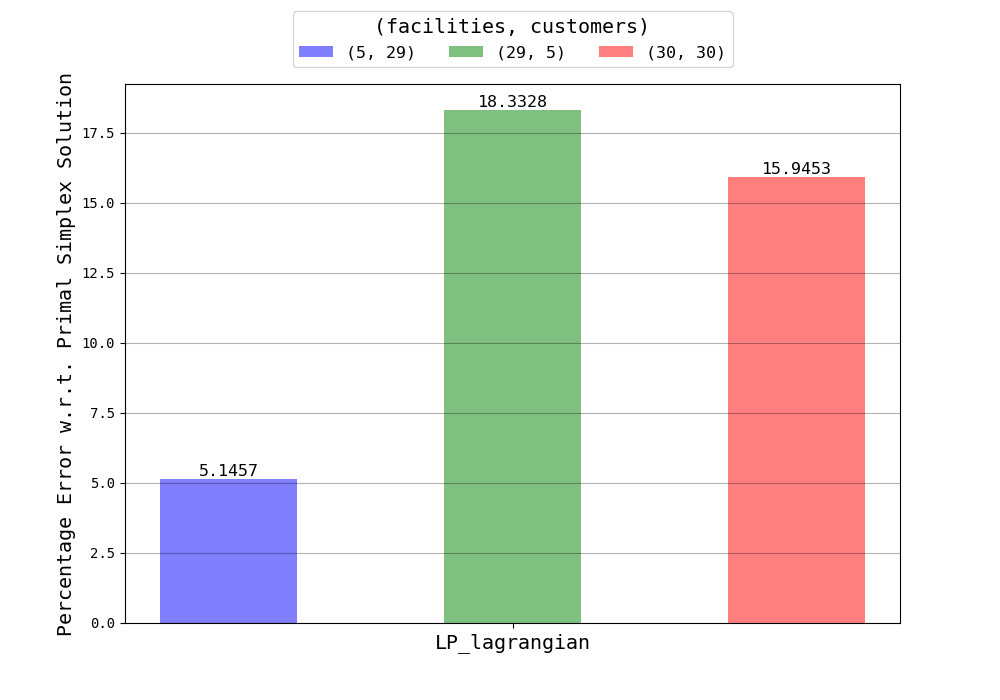
\includegraphics[width=6.5cm,height=4.2cm]{img/chart_error_lagrangian_4.png}
        
        \centering
        \column{.5\textwidth}
        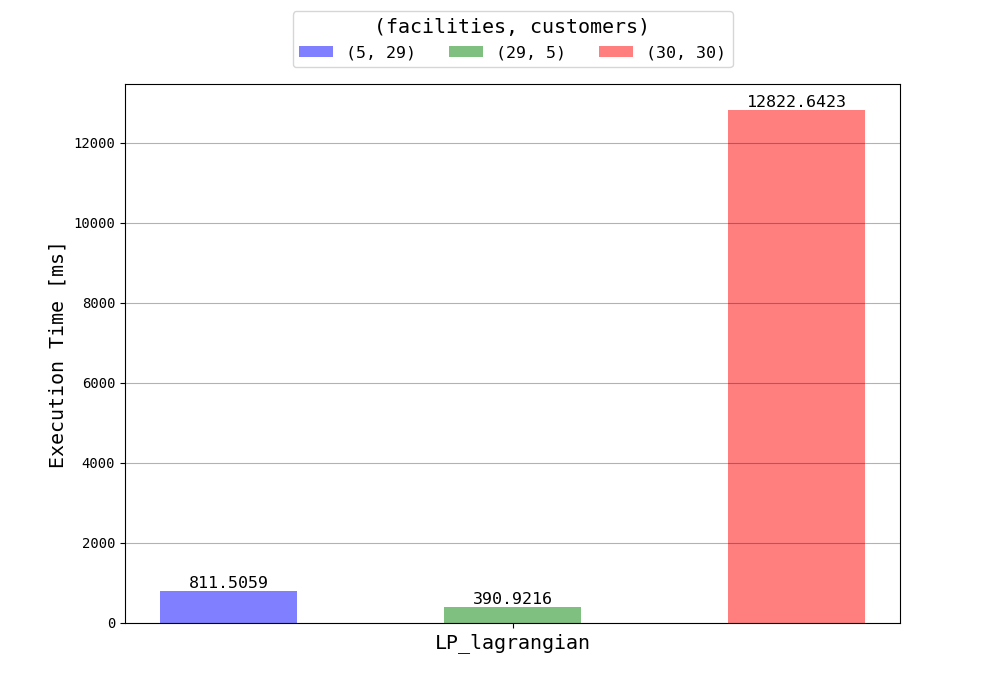
\includegraphics[width=6.5cm,height=4.2cm]{img/chart_time_lagrangian_4.png}
        \end{columns}
        
	    \end{frame}
	
	\section{Conclusion}
	\begin{frame}{Conclusion (1)}
	
	Best algorithms in \textbf{percentage errors}:
	\begin{table}
	\begin{tabular}{| l | ccc |}
	\hline
     & (5, 29) & (29, 5) & (30, 30) \\
    \hline
        \rowcolor{shadecolor}
        Test case 1 & \textit{Linear r.} & \textit{Linear r.} & \textit{Linear r.} \\
        Test case 2 & \textit{Linear r.} & \textit{Linear r.} & \textit{Linear r.} \\
        \rowcolor{shadecolor}
        Test case 3 & \textit{Linear r.} & \textit{Linear r.} & \textit{Dualoc} \\
        Test case 4 & \textit{Lagrangian r.} & \textit{Dualoc} & \textit{Linear r.} \\
        \rowcolor{shadecolor}
        Test case 5 & \textit{Linear r.} & \textit{Dualoc} & \textit{Linear r.} \\
    \hline
        
    \end{tabular}
    \end{table}
    
    \begin{itemize}
        \item \textit{11} times \textit{Linear relaxation} provides the minimum error
        \item \textit{3} times \textit{Dualoc} provides the minimum error
        \item \textit{1} times \textit{Lagrangian relaxation} provides the minimum error
    \end{itemize}
    
	\end{frame}
	
	\begin{frame}{Conclusion (2)}
	
	Best algorithms in \textbf{computation times}:
	
	\begin{table}
	\begin{tabular}{| l | ccc |}
	\hline
     & (5, 29) & (29, 5) & (30, 30) \\
    \hline
        \rowcolor{shadecolor}
        Test case 1 & \textit{Dualoc} & \textit{Dualoc} & \textit{Linear r.} \\
        Test case 2 & \textit{Dualoc} & \textit{Dualoc} & \textit{Linear r.} \\
        \rowcolor{shadecolor}
        Test case 3 & \textit{Dualoc} & \textit{Dualoc} & \textit{Linear r.} \\
        Test case 4 & \textit{Dualoc} & \textit{Dualoc} & \textit{Linear r.} \\
        \rowcolor{shadecolor}
        Test case 5 & \textit{Dualoc} & \textit{Dualoc} & \textit{Dualoc} \\
    \hline
    \end{tabular}
    \end{table}
    
    \begin{itemize}
        \item \textit{4} times \textit{Linear relaxation} provides the minimum time
        \item \textit{11} times \textit{Dualoc} provides the minimum time
    \end{itemize}
    
	\end{frame}
\end{document}